\subsection{经典机器学习算法}
\subsubsection{从logit模型开始}
\begin{frame}[fragile]
    \frametitle{logit 模型}
    关于分类我们自然地想到了 logit 回归。我们不妨以 logit 回归为切入点看一看 sklearn 是如何训练模型的:

    \begin{minted}{python}
from sklearn.linear_model import LogisticRegression
logit = LogisticRegression(solver="saga",
            multi_class="multinomial", random_state=42)
logit.fit(Xtrain, Ytrain)
logit.predict(Xtest)
    \end{minted}

    \begin{table}
        \caption{logit 回归}
        \begin{tabular}{ll}
            precision & 0.1815  \\
            recall    & 0.2440  \\
            f1        & 0.1547  \\
            \(R^2\)   & -0.0177 \\
        \end{tabular}
        \label{logit}
    \end{table}
\end{frame}
\subsubsection{基于树的算法}
\begin{frame}[fragile]
    \frametitle{决策树}

    决策树直观上很好理解,也是我们今天少数可解释的模型。一个数据集有多个特征,每个节点按照某个特征是否满足一定的条件分叉,形成一棵二叉树。

    该节点选取特征分叉的决策依据是最大化“信息增益”,即分叉前后数据更“有序”,且更有序的程度最大(信息熵变化最大)。
    这棵树为了避免过拟合,我们会对决策树“剪枝”,增加一些分支条件的限制,可以看\href{https://scikit-learn.org/stable/modules/generated/sklearn.tree.DecisionTreeClassifier.html}{sklearn 文档}。
    \begin{center}
        \begin{figure}
            \includegraphics[width=0.8\linewidth]{/Users/dcy/Desktop/thesis/data/decision_tree.png}
            \label{decisiontree}
            \caption{决策树}
        \end{figure}
    \end{center}
\end{frame}
\begin{frame}
    \frametitle{集成学习}
    决策树一般是一种比较弱的分类器。集成学习则是利用多个弱分类器的集成,形成一个强分类器。

    组合的方法常见的有两种:bagging 和 boosting。bagging 是平行地训练弱分类器然后投票,特点是不容易过拟合。
    典型的随机森林就是随机地选取样本和特征训练出一棵棵决策树后投票,如图 \ref{randomforest} 所示。
    \begin{center}
        \begin{figure}
            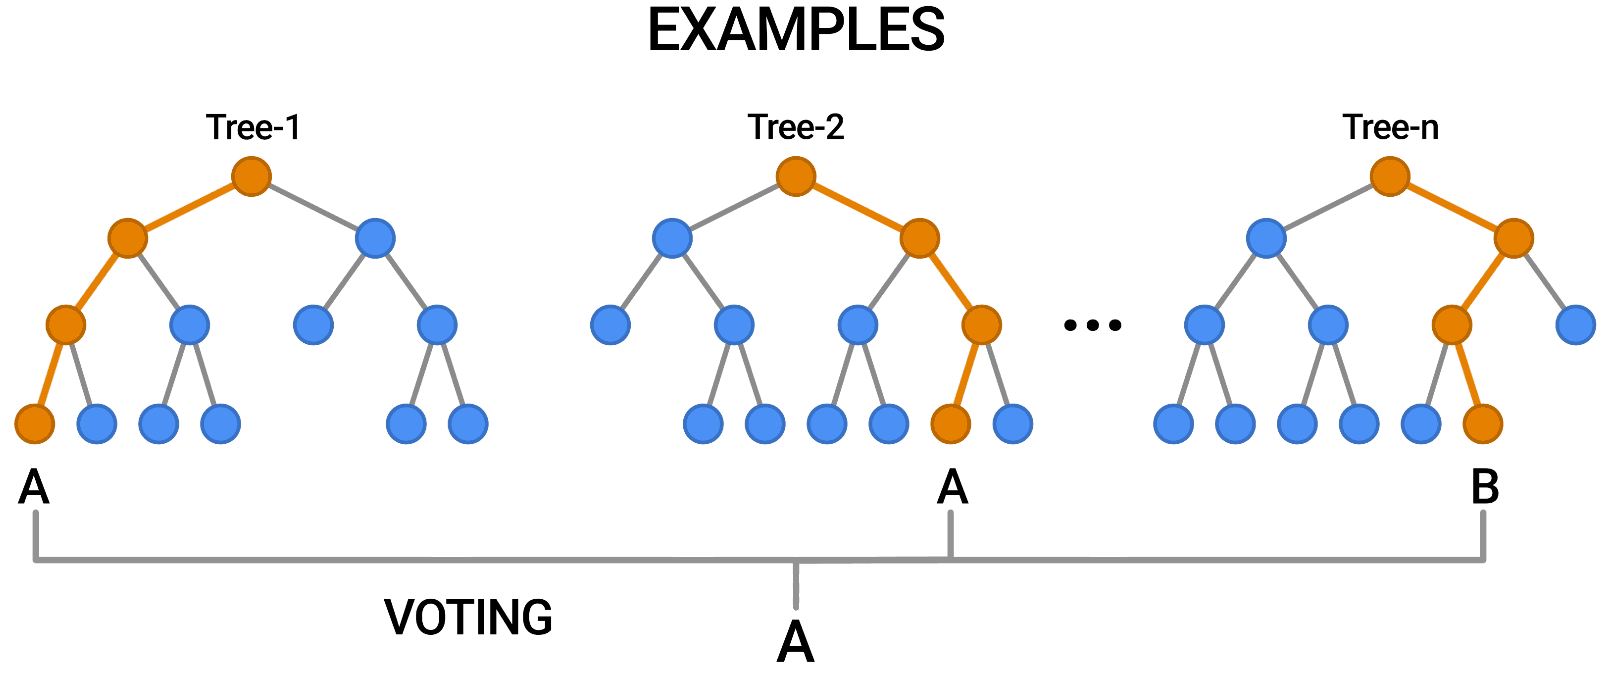
\includegraphics[width=0.8\linewidth]{../lib/rf.png}
            \label{randomforest}
            \caption{随机森林}
        \end{figure}
    \end{center}
\end{frame}
\begin{frame}
    \frametitle{集成学习}
    使用 boosting 的梯度提升树可以树的深度很少就能达到很高的精度。
    boosting 迭代地训练一系列的分类器,每个分类器采用的样本分布都和上一轮的学习结果有关,直观比方是每个树都去学习上一个树没有学习好的地方。
    \begin{center}
        \begin{figure}
            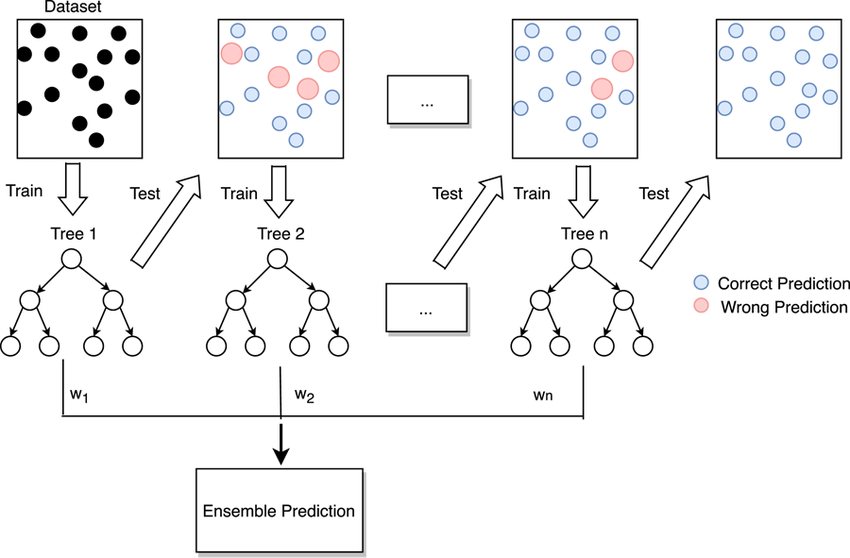
\includegraphics[width=0.6\linewidth]{../lib/boosting.png}
            \label{boosting}
            \caption{梯度提升树}
        \end{figure}
    \end{center}
\end{frame}
\begin{frame}[fragile]
    \frametitle{基于树的算法代码}
    \begin{minted}{python}
from sklearn.tree import DecisionTreeClassifier
from sklearn.ensemble import RandomForestClassifier
from sklearn.ensemble import GradientBoostingClassifier
dt = DecisionTreeClassifier(max_depth=3, random_state=42)
dt.fit(Xtrain, Ytrain)
rf = RandomForestClassifier(max_depth=4, random_state=42)
rf.fit(Xtrain, Ytrain)
gb = GradientBoostingClassifier(max_depth=3, random_state=42)
gb.fit(Xtrain, Ytrain)
    \end{minted}
    \begin{table}
        \caption{基于树的算法结果}
        \begin{tabular}{l|cccc}
            model & precision & recall & f1     & \(R^2\) \\ \hline
            决策树   & 0.3498    & 0.3799 & 0.3529 & 0.3632  \\
            随机森林  & 0.3960    & 0.4251 & 0.3835 & 0.3995  \\
            梯度提升树 & 0.5305    & 0.5256 & 0.5095 & 0.5421  \\
        \end{tabular}
        \label{trees}
    \end{table}
\end{frame}
\subsubsection{基于距离的算法}
\begin{frame}
    \frametitle{支持向量机}
    SVM 的思想是样本分布在空间中,找到一个可以恰好划分开样本点、并且间隔最大的的(超)平面。

    当然这样的超平面不一定好找,我们可以用加入惩罚项的“软间隔”优化或者利用“核函数”将空间映射为可分的。

    \begin{center}
        \begin{figure}
            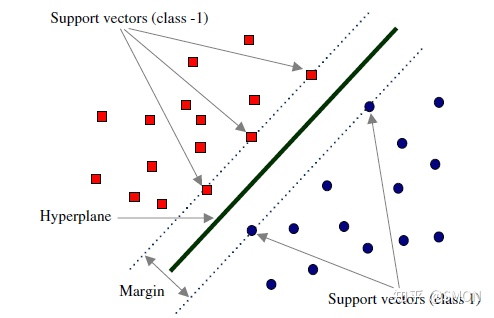
\includegraphics[width=0.6\linewidth]{../lib/SVM.jpeg}
            \caption{Support Vector Machine}
            \label{SVM}
        \end{figure}
    \end{center}
\end{frame}
\begin{frame}
    \frametitle{KNN 与 K Means}
    \begin{columns}
        \column{0.5\linewidth}
        KNN 的思想是一个样本归属的分类属于离他最近的 K 个已经打好标签的邻居中占多数的分类,也非常直观。
        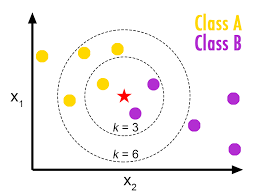
\includegraphics[width=0.9\linewidth]{../lib/KNN.png}
        \column{0.5\linewidth}
        K Means 则是一种聚类算法,不需要打好标签(即所谓“无监督学习”),目的是把样本点归为 K 个群落。
        其思想是假设 K 个重心,样本根据与不同重心的距离归类,进而得到新的重心。
        以此循环往复,直至重心稳定下来。
        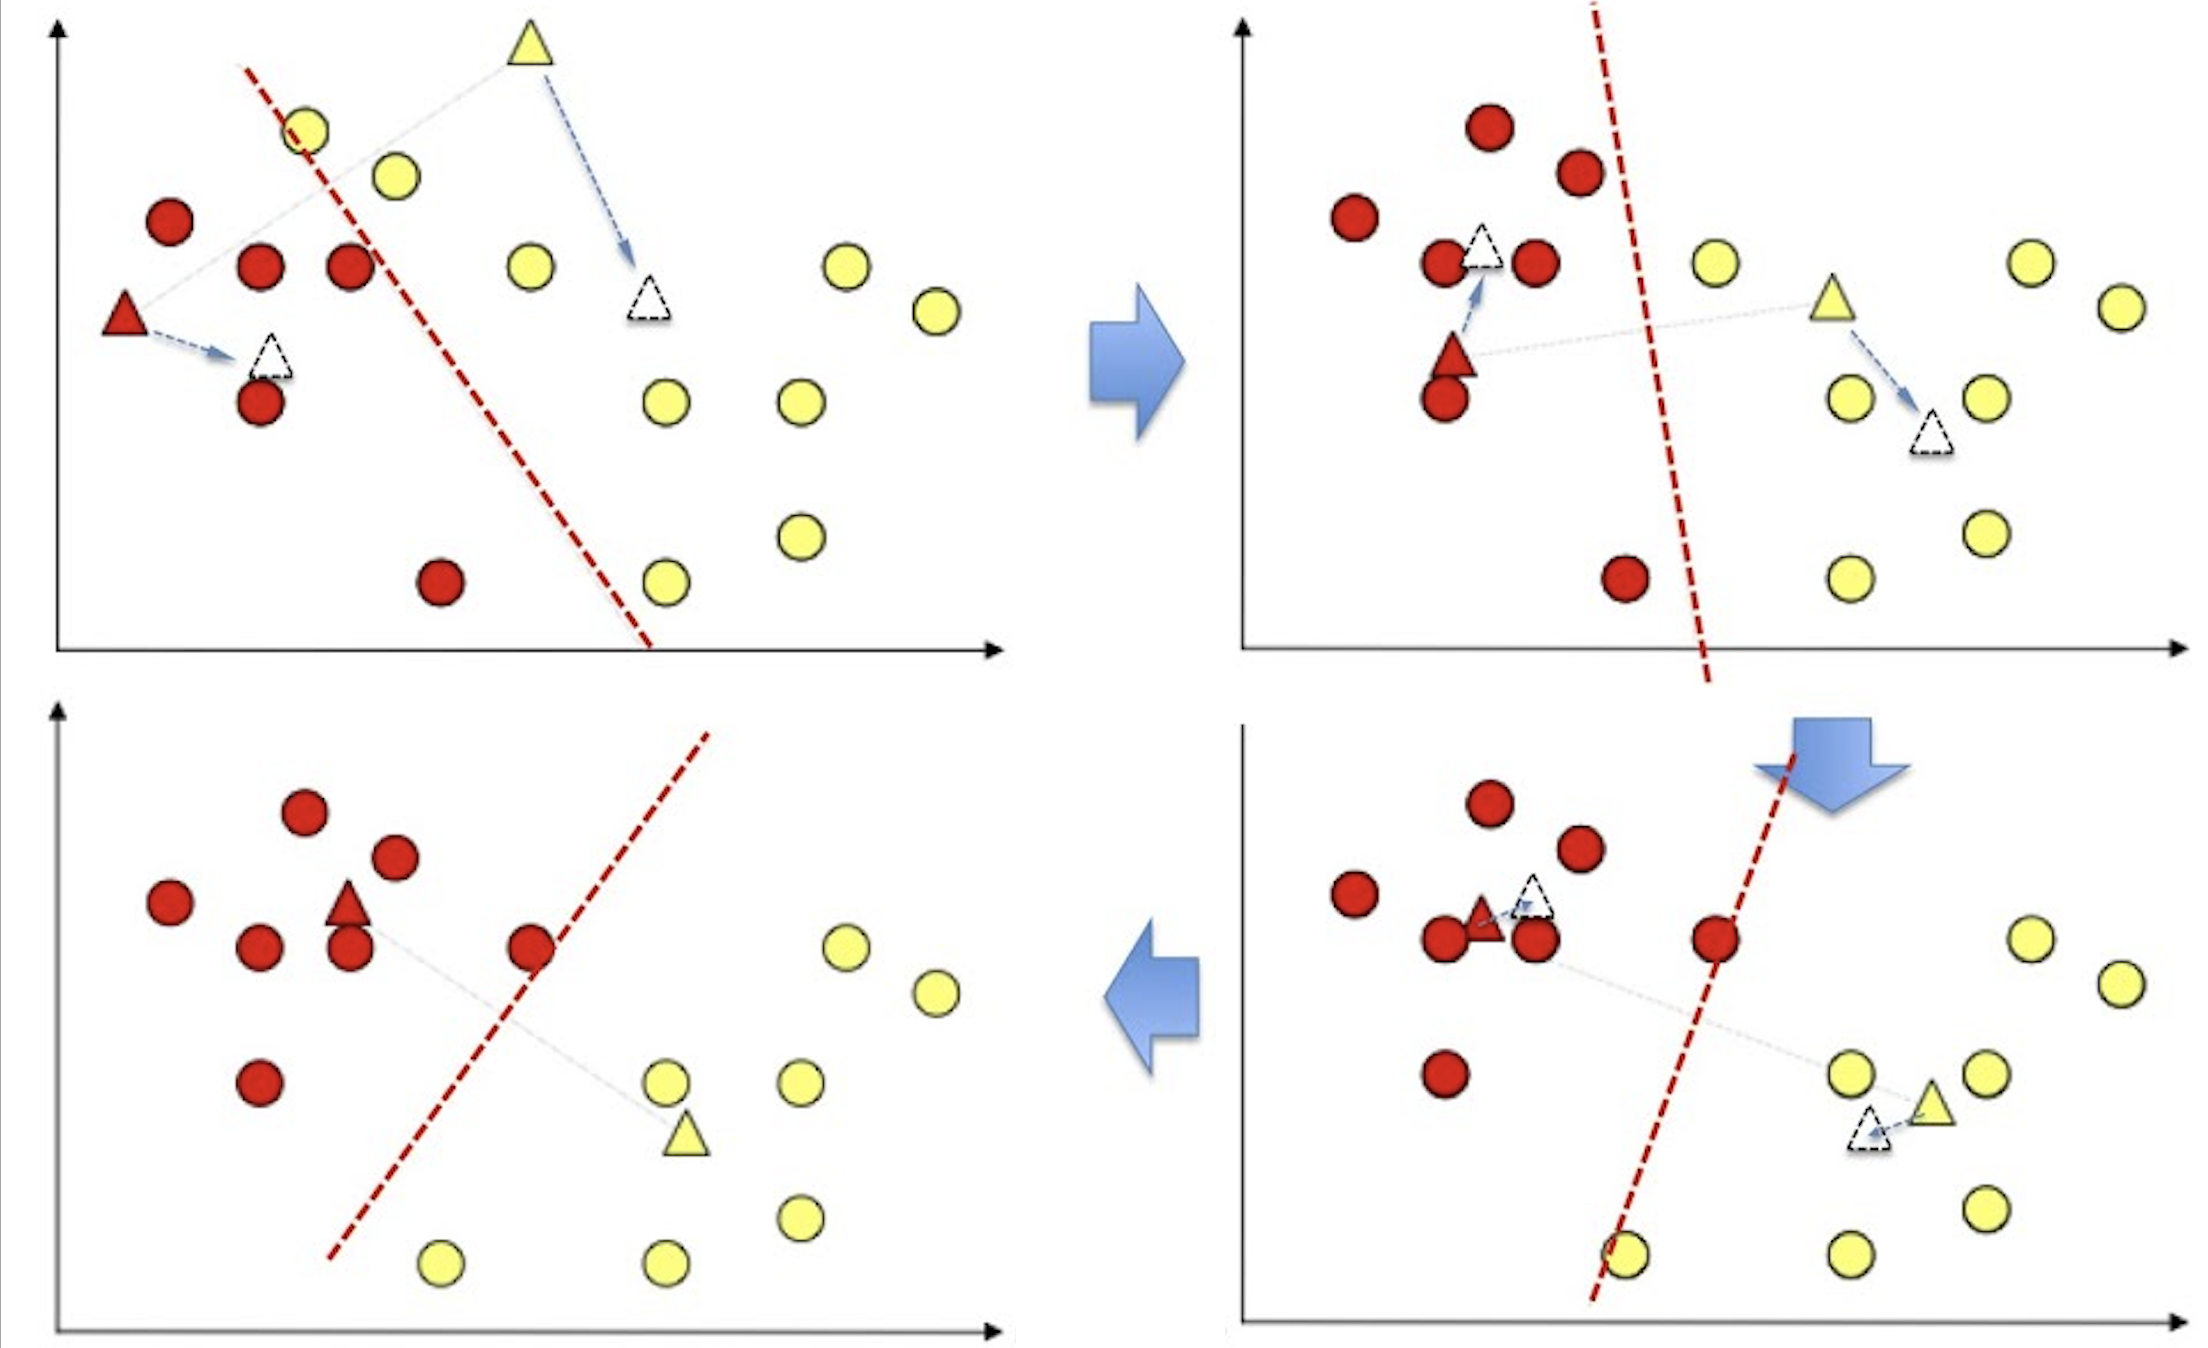
\includegraphics[width=0.9\linewidth]{../lib/kmeans.png}
    \end{columns}
\end{frame}
\begin{frame}[fragile]
    \frametitle{基于距离的算法实现}
    \begin{minted}{python}
from sklearn.neighbors import KNeighborsClassifier
from sklearn.svm import SVC

svm = SVC(kernel="rbf", gamma="auto", random_state=42)
svm.fit(Xtrain, Ytrain)
KNN = KNeighborsClassifier(n_neighbors=3)
KNN.fit(Xtrain, Ytrain)
    \end{minted}
    \begin{table}
        \caption{基于距离的算法结果}
        \begin{tabular}{l|cccc}
            model & precision & recall & f1     & \(R^2\) \\ \hline
            SVM   & 0.4137    & 0.4094 & 0.3517 & 0.3431  \\
            KNN   & 0.3625    & 0.3523 & 0.3420 & 0.2987  \\
        \end{tabular}
        \label{distances}
    \end{table}
\end{frame}
\subsection{对比}
\begin{frame}
    \frametitle{结果对比}
    \centering
    \begin{table}
        \caption{机器学习效果对比表}
        \label{result}
        \begin{tabular}{l|cccc}
            model    & precision & recall & f1     & \(R^2\) \\\hline
            random   & 0.2364    & 0.1255 & 0.1544 & 0.0089  \\
            logit    & 0.1815    & 0.2441 & 0.1547 & -0.0178 \\
            tree     & 0.3499    & 0.3799 & 0.3529 & 0.3632  \\
            bagging  & 0.3960    & 0.4252 & 0.3835 & 0.3996  \\
            boosting & 0.5305    & 0.5256 & 0.5095 & 0.5421  \\
            svm      & 0.4137    & 0.4094 & 0.3517 & 0.3431  \\
            KNN      & 0.3625    & 0.3524 & 0.342  & 0.2987  \\
            BP       & 0.3035    & 0.3267 & 0.2913 & 0.0463  \\
            CNN      & 0.4027    & 0.4350 & 0.4140 & 0.4039  \\
            RNN      & 0.4516    & 0.4606 & 0.4541 & 0.4176  \\
        \end{tabular}
    \end{table}

\end{frame}
\begin{frame}
    \frametitle{结果对比}
    \centering
    \begin{figure}
        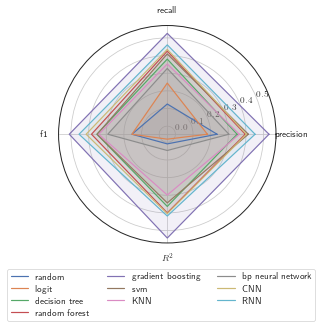
\includegraphics[width=0.5\linewidth]{../lib/output.png}
        \caption{机器学习效果对比图}
        \label{contrast}
    \end{figure}
\end{frame}
\section{机器学习在企业风险管理中的应用}

\begin{frame}
    \frametitle{机器学习在企业风险管理中的应用}
    \Textcite{mai2019deep} 利用 CNN 预测企业破产,在处理文本数据时利用 word embedding 量化,AUC 曲线如图
    \begin{figure}
        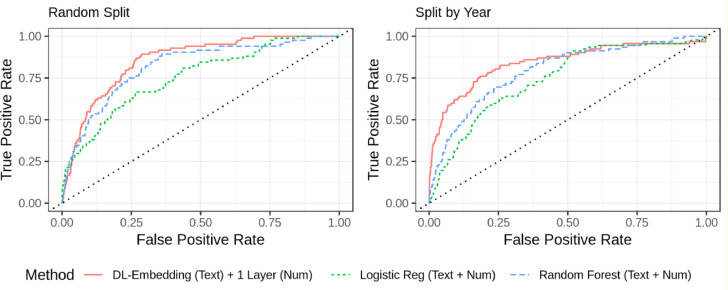
\includegraphics[width=\linewidth]{../lib/mlinerm.jpg}
        \caption{AUC曲线}
    \end{figure}
\end{frame}
\begin{frame}
    \frametitle{机器学习在企业风险管理中的应用}
    \Textcite{kellner2022opening} 利用神经网络预测违约损失 Loss Given Default。

    他们将传统的分位数回归的回归元作为第一层,通过神经网络揭示其中的非线性关系,比如交叉项及其他非线性关系,神经网络最后一层是传统的分位数回归。利用 first order feature importance,量化输入变量的整体重要性。同时排除掉二阶的和交互的在分位数中接近于零。因此 QRNN 和分位数 QR 的分位数损失非常相似
    通过允许分位数回归神经网络实现的分位数中的非线性和相互作用来扩展这种方法。这种方法大大增强了建模的灵活性。额外的灵活性在更好地分布拟合和超时样本方面带来了回报,分位数预测精度提高了 30\%,同时更加 robust 。
\end{frame}
\begin{frame}
    \frametitle{机器学习在企业风险管理中的应用}
    \Textcite{golbayani2020comparative}
    使用决策树、随机森林、支持向量机和多层感知器应用于相同的数据集,预测公司未来评级。他们统计了机器学习在债券评级和公司信用评级方面的文章,很多认为 SVM
    和神经网络是比较准确的。但是他们使用 Notches Distance 来对机器学习绩效来打分,认为基于决策树的两种方法更有效。

    当前机器学习最火热的两个应用方向是计算机视觉 CV 和自然语言处理 NLP ,亦有一些文献利用自然语言处理分析文本数据做研究。
\end{frame}

